% The flow in artifact terms: stages, the tool that runs each one, and the
% files it writes. Single column, top to bottom, two inputs and one fan-out.
\documentclass[border=4pt]{standalone}
\usepackage{tikz}
\usetikzlibrary{arrows.meta, positioning, calc}
\usepackage[T1]{fontenc}
\usepackage{lmodern}

\definecolor{IHPfg}{RGB}{0,80,139}
\definecolor{IHPaccent}{RGB}{109,112,114}
\definecolor{IHPgreen}{RGB}{65,155,75}
\definecolor{cKicad}{RGB}{0,80,139}
\definecolor{cChiplet}{RGB}{55,145,195}
\definecolor{cGDS2K}{RGB}{228,15,19}
\definecolor{cDesigns}{RGB}{120,70,150}

\begin{document}
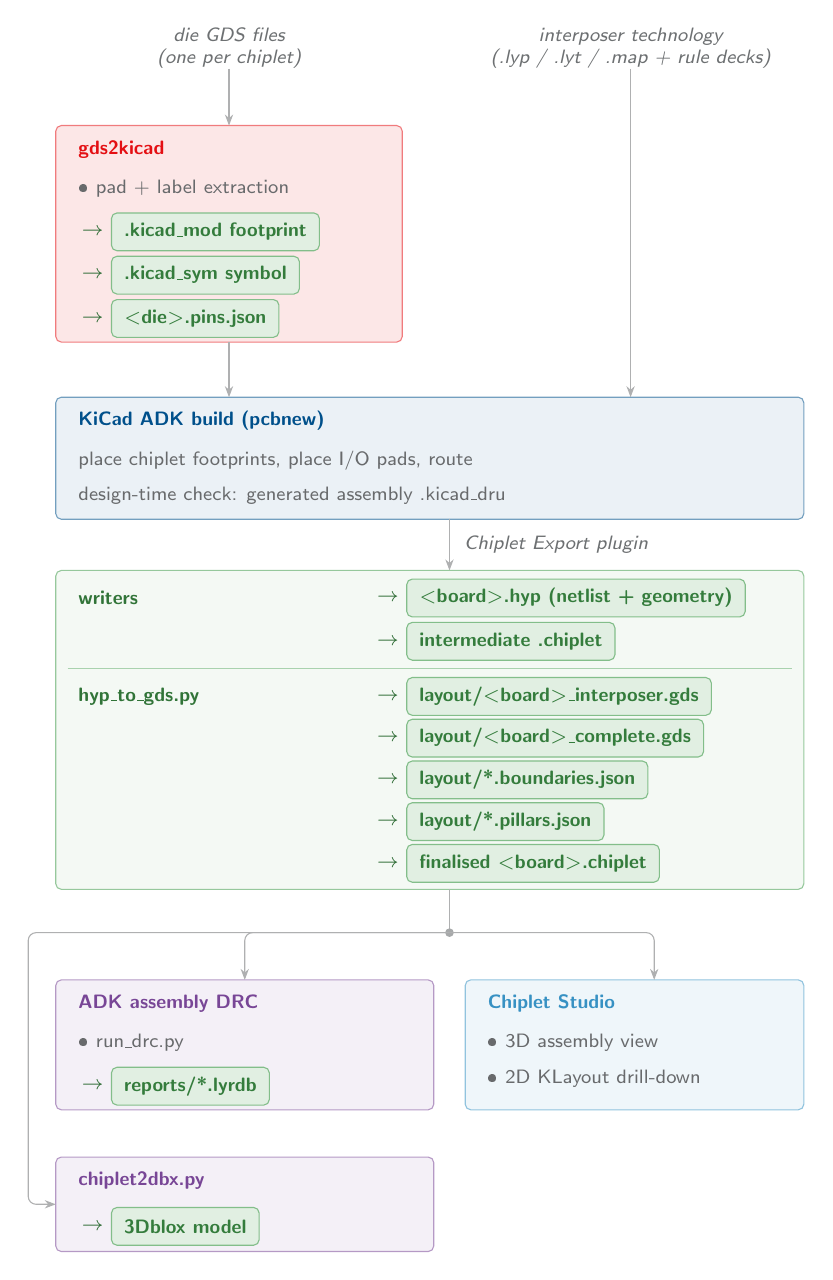
\begin{tikzpicture}[
    >=Stealth,
    adkframe/.style={
        rounded corners=2pt, draw=#1!55, fill=#1!8, line width=0.4pt
    },
    adktitle/.style={
        font=\sffamily\scriptsize\bfseries, text=#1, inner sep=0pt
    },
    adkbody/.style={
        font=\sffamily\scriptsize, text=IHPaccent!95!black, inner sep=0pt
    },
    adkin/.style={
        font=\sffamily\scriptsize\itshape, text=IHPaccent, align=center,
        inner sep=0pt
    },
    adkanno/.style={
        font=\sffamily\scriptsize\itshape, text=IHPaccent, inner sep=0pt
    },
    adkout/.style={
        rounded corners=2pt,
        draw=IHPgreen!65, fill=IHPgreen!16, line width=0.4pt,
        minimum height=4.8mm, inner xsep=1.6mm, inner ysep=0.6mm,
        font=\sffamily\scriptsize\bfseries, text=IHPgreen!80!black
    },
    adktick/.style={
        font=\sffamily\scriptsize, text=IHPgreen!70!black, inner sep=0pt
    },
    adkarrow/.style={
        -{Stealth[length=1.4mm]}, line width=0.4pt, color=IHPaccent!55,
        rounded corners=1mm
    },
    adkline/.style={
        line width=0.4pt, color=IHPaccent!55
    }
]

% ===================== frames =====================
\draw[adkframe=cGDS2K, fill=cGDS2K!10] (-5.00,-0.80) rectangle (-0.60,-3.55);
\draw[adkframe=cKicad]                 (-5.00,-4.25) rectangle ( 4.50,-5.80);
\draw[adkframe=IHPgreen, fill=IHPgreen!6]
                                       (-5.00,-6.45) rectangle ( 4.50,-10.50);
\draw[adkframe=cDesigns]               (-5.00,-11.65) rectangle (-0.20,-13.30);
\draw[adkframe=cChiplet]               ( 0.20,-11.65) rectangle ( 4.50,-13.30);
\draw[adkframe=cDesigns]               (-5.00,-13.90) rectangle (-0.20,-15.10);

% divider between the two halves of the export stage
\draw[line width=0.3pt, color=IHPgreen!45] (-4.85,-7.70) -- (4.35,-7.70);

% ===================== inputs =====================
\node[adkin, anchor=north] (inl) at (-2.80, 0.45)
    {die GDS files\\(one per chiplet)};
\node[adkin, anchor=north] (inr) at ( 2.30, 0.45)
    {interposer technology\\(.lyp / .lyt / .map + rule decks)};

% ===================== arrows =====================
\draw[adkarrow] (inl.south) -- (-2.80,-0.80);
\draw[adkarrow] (inr.south) -- ( 2.30,-4.25);
\draw[adkarrow] (-2.80,-3.55) -- (-2.80,-4.25);
\draw[adkarrow] ( 0.00,-5.80) -- ( 0.00,-6.45);
\draw[adkline]  ( 0.00,-10.50) -- ( 0.00,-11.05);
\fill[IHPaccent!60] (0.00,-11.05) circle (0.055);
\draw[adkarrow] ( 0.00,-11.05) -| (-2.60,-11.65);
\draw[adkarrow] ( 0.00,-11.05) -| ( 2.60,-11.65);
% chiplet2dbx.py reads the finalised .chiplet, not the DRC report, so it is a
% third consumer of the export stage rather than a stage downstream of the DRC.
\draw[adkarrow] ( 0.00,-11.05) -| (-5.35,-14.50) -- (-5.00,-14.50);

\node[adkanno, anchor=west] at (0.18,-6.12) {Chiplet Export plugin};

% ===================== gds2kicad =====================
\node[adktitle=cGDS2K, anchor=west] at (-4.72,-1.10) {gds2kicad};
\node[adkbody, anchor=west] at (-4.72,-1.60) {\textbullet~pad + label extraction};

\node[adktick, anchor=west] at (-4.68,-2.15) {$\rightarrow$};
\node[adkout,  anchor=west] at (-4.30,-2.15) {.kicad\_mod footprint};
\node[adktick, anchor=west] at (-4.68,-2.70) {$\rightarrow$};
\node[adkout,  anchor=west] at (-4.30,-2.70) {.kicad\_sym symbol};
\node[adktick, anchor=west] at (-4.68,-3.25) {$\rightarrow$};
\node[adkout,  anchor=west] at (-4.30,-3.25) {\textless{}die\textgreater{}.pins.json};

% ===================== KiCad ADK build =====================
\node[adktitle=cKicad, anchor=west] at (-4.72,-4.55) {KiCad ADK build (pcbnew)};
\node[adkbody, anchor=west] at (-4.72,-5.05)
    {place chiplet footprints, place I/O pads, route};
\node[adkbody, anchor=west] at (-4.72,-5.50)
    {design-time check: generated assembly .kicad\_dru};

% ===================== writers + hyp_to_gds =====================
\node[adktitle=IHPgreen!75!black, anchor=west] at (-4.72,-6.80) {writers};
\node[adktick, anchor=west] at (-0.93,-6.80) {$\rightarrow$};
\node[adkout,  anchor=west] at (-0.55,-6.80)
    {\textless{}board\textgreater{}.hyp (netlist + geometry)};
\node[adktick, anchor=west] at (-0.93,-7.35) {$\rightarrow$};
\node[adkout,  anchor=west] at (-0.55,-7.35) {intermediate .chiplet};

\node[adktitle=IHPgreen!75!black, anchor=west] at (-4.72,-8.05) {hyp\_to\_gds.py};
\node[adktick, anchor=west] at (-0.93,-8.05) {$\rightarrow$};
\node[adkout,  anchor=west] at (-0.55,-8.05)
    {layout/\textless{}board\textgreater{}\_interposer.gds};
\node[adktick, anchor=west] at (-0.93,-8.58) {$\rightarrow$};
\node[adkout,  anchor=west] at (-0.55,-8.58)
    {layout/\textless{}board\textgreater{}\_complete.gds};
\node[adktick, anchor=west] at (-0.93,-9.11) {$\rightarrow$};
\node[adkout,  anchor=west] at (-0.55,-9.11) {layout/*.boundaries.json};
\node[adktick, anchor=west] at (-0.93,-9.64) {$\rightarrow$};
\node[adkout,  anchor=west] at (-0.55,-9.64) {layout/*.pillars.json};
\node[adktick, anchor=west] at (-0.93,-10.17) {$\rightarrow$};
\node[adkout,  anchor=west] at (-0.55,-10.17)
    {finalised \textless{}board\textgreater{}.chiplet};

% ===================== assembly DRC =====================
\node[adktitle=cDesigns, anchor=west] at (-4.72,-11.95) {ADK assembly DRC};
\node[adkbody, anchor=west] at (-4.72,-12.45) {\textbullet~run\_drc.py};
\node[adktick, anchor=west] at (-4.68,-13.00) {$\rightarrow$};
\node[adkout,  anchor=west] at (-4.30,-13.00) {reports/*.lyrdb};

% ===================== Chiplet Studio =====================
\node[adktitle=cChiplet, anchor=west] at (0.48,-11.95) {Chiplet Studio};
\node[adkbody, anchor=west] at (0.48,-12.45) {\textbullet~3D assembly view};
\node[adkbody, anchor=west] at (0.48,-12.90) {\textbullet~2D KLayout drill-down};

% ===================== chiplet2dbx =====================
\node[adktitle=cDesigns, anchor=west] at (-4.72,-14.20) {chiplet2dbx.py};
\node[adktick, anchor=west] at (-4.68,-14.78) {$\rightarrow$};
\node[adkout,  anchor=west] at (-4.30,-14.78) {3Dblox model};

\end{tikzpicture}
\end{document}
